%!TEX root = main.tex

\chapter{Microsoft Quantum Development Kit}
\label{chp:qdk}

QDK is Microsoft's open source developement kit for quantum computing. It is quite young, as it has been released in January 2018. Despite that, it has some interesting characteristics, like the use of a specific ``quantum focused'' language: Q\#. Differently from  other frameworks (like pyQuil, QISKit, ProjectQ...), QDK uses a technology based on Majorana fermions, which is also the reason why right now there are no hardware devices on which run the algorithms. \cite{larose2019overview}

It is updated very frequently with often drastic improvement in terms of usability and bug fixes. Of course it is not yet a mature enviroment, as it is still under development.

\section{Software overview}

\subsection{Installation}

Microsoft QDK can be installed on top of Visual Studio or Visual Studio Code (recommended). The setup is easy and the process it's well explained in the official page: \url{https://docs.microsoft.com/it-it/quantum/install-guide/vs-2017}.

After installation it is also possible to validate its correctness running a sample program whose aim is to check the possible absence of needed packages (linke NuGet).

\subsection{Documentation}

A complete documentation of the software and language can be found on the official website \url{https://docs.microsoft.com/it-it/quantum}. It contains tutorials on how to run the first quantum program, info about the simulator, Q\# syntax and its libraries. Other part of the website also contain a good documentation on the theory about quantum computing.

Moreover the open source libraries are useful to learn the language. Last but not least, there is a vast number of verbosely commented examples (Teleportation, Grover's Search, Integer factorization, simulations...).

\subsection{Language Q\#}

Using QDK requires some basic knowledge of C\# for the classical host computation, usually contained in a ``driver.cs'' file, that is used to call the simulator with the quantum program, optionally providing inputs.

The quantum part of the program uses Q\# that, despite the name, is more similar to a hardware description language than to an object oriented one. We can define \textit{operations}, callable routines with quantum instructions, that as functions take some input and return an output value. We can also define variables to values bindings (like integers and booleans), perform operations on single qubits (like gates, conditionals and controls).

In general the language is high level oriented: you do not have to design the spatial disposition of gates on qubit lines as you are not bound to a specific architecture, therefore the programmer can focus more on the algorithm than on the implementation details, thanks also to the available libraries.

\subsection{Simulator}

QDK can be used within a local run of Visual Studio, in this case it can simulate circuits of up to 30 qubits. If more power is needed, it can also be run in Microsoft Azure cloud (through a pais subscription) achieving simulations of more than 40 qubits.

It uses a locally deployed simulation environment based on dotnet. The language abstracts from the actual architecture to be deployed (it uses Qubit objects, not specific low level registers), in order to allow an better re-usability and portability of the code.

It also implements a Toffoli simulator, a special-purpose simulator for quantum algorithms that are limited to X, CNOT, and multi-controlled X.

A trace simulator is also provided. It is useful for debugging classical code and estimating the resources required to run a given instance of a quantum program. Circuits of thousands of qubits can be tested, as the trace simulator executes the program without simulating the state of the quantum computer.

\subsubsection{Hardware and noise analysis}

The technology Microsoft is trying to use has not been implemented on hardware yet. Moreover QDK does not provide any functionality for noise analysis or simulation. This is probably connected to the fact that Microsoft is betting on topological qubits, that should be highly resilient to noise and decoherence.

\section{Sample Q\# code: Grover Search}
\label{sec:QSgrover}

\lstset{
	language=qsharp,
	basicstyle=\scriptsize
}

QDK comes with a bunch of code samples to help the user understanding the basics of the language and its potentialities. Among these examples we want to mention \textit{qubits teleportation}, \textit{CHSH Game}, \textit{Grover's Algorithm} (called Database Search) and Integer factorization.

\bigskip

In this document we are not going to describe the details of Grover's Algorithm in function, as it is not our purpose (for this please refer to \cite{Grover:1996:FQM:237814.237866}). However it's instructive to read some examples of Q\# code, so let's take a quick look at Grover's Algorithm implementation.

\begin{lstlisting}
/// This sample will walk through several examples of searching a database of N elements for a particular marked item using just O(1/√N) queries to the database. [...] We will model the database by an oracle D that acts to map indices to a flag indicating whether a given index is marked.
/// [...]
/// (it) makes full use of the amplitude amplification library and other supporting libraries to implement Grover's algorithm more easily. We also consider a more general instance of the database oracle that allows us to mark multiple elements.
\end{lstlisting}

For a simpler and less theory requiring example of Q\# code see also \cref{sec:qs_impl}.

\subsection{The code}

\begin{lstlisting}
// Copyright (c) Microsoft Corporation. All rights reserved.
// Licensed under the MIT License.
\end{lstlisting}

\noindent First an oracle D is built from the classical database

\begin{lstlisting}
operation DatabaseOracleFromInts (markedElements : Int[], markedQubit : Qubit, databaseRegister : Qubit[]) : Unit {

	body (...) {
		let nMarked = Length(markedElements);
		
		for (idxMarked in 0 .. nMarked - 1) {
			(ControlledOnInt(markedElements[idxMarked], ApplyToEachCA(X, _)))(databaseRegister, [markedQubit]);
		}
	}
	
	adjoint invert;
	controlled distribute;
	controlled adjoint distribute;
}
\end{lstlisting}

\noindent Then we prepare the state oracle

\begin{lstlisting}
operation GroverStatePrepOracleImpl (markedElements : Int[], idxMarkedQubit : Int, startQubits : Qubit[]) : Unit {

	body (...) {
		let flagQubit = startQubits[idxMarkedQubit];
		let databaseRegister = Exclude([idxMarkedQubit], startQubits);
		
		// Apply oracle `U`
		ApplyToEachCA(H, databaseRegister);
		
		// Apply oracle `D`
		DatabaseOracleFromInts(markedElements, flagQubit, databaseRegister);
	}
	
	adjoint invert;
	controlled distribute;
	controlled adjoint distribute;
}
\end{lstlisting}

\noindent Finally the library function `AmpAmpByOracle' returns a unitary that implements all steps of Grover's algorithm.

\begin{lstlisting}
function GroverSearch (markedElements : Int[], nIterations : Int, idxMarkedQubit : Int) : (Qubit[] => Unit : Adjoint, Controlled) {

	return AmpAmpByOracle(nIterations, GroverStatePrepOracle(markedElements), idxMarkedQubit);
}
\end{lstlisting}

\noindent Putting all together

\begin{lstlisting}
operation ApplyGroverSearch (markedElements : Int[], nIterations : Int, nDatabaseQubits : Int) : (Result, Int) {
	
	// Allocate variables to store measurement results.
	mutable resultSuccess = Zero;
	mutable numberElement = 0;
	
	// Allocate nDatabaseQubits + 1 qubits. These are all in the |0〉
	// state.
	using (qubits = Qubit[nDatabaseQubits + 1]) {
		
		// Define marked qubit to be indexed by 0.
		let markedQubit = qubits[0];
		
		// Let all other qubits be the database register.
		let databaseRegister = qubits[1 .. nDatabaseQubits];
		
		// Implement the quantum search algorithm.
		(GroverSearch(markedElements, nIterations, 0))(qubits);
		
		// Measure the marked qubit. On success, this should be One.
		set resultSuccess = M(markedQubit);
		
		// Measure the state of the database register post-selected on
		// the state of the marked qubit.
		let resultElement = MultiM(databaseRegister);
		set numberElement = PositiveIntFromResultArr(resultElement);
		
		// These reset all qubits to the |0〉 state, which is required
		// before deallocation.
		ResetAll(qubits);
	}
	
	// Returns the measurement results of the algorithm.
	return (resultSuccess, numberElement);
}
\end{lstlisting}

\subsection{Results of multiple runs of the code}

We performed some runs of the algorithm, shaping the output so that it could be easy intelligible. In particular, to show the potentialities of Grover's Search and the theoretical speedup with respect to the classical one we collected stats on:
\begin{itemize}
	\item classical search of one element in \cref{fig:db_stats1}
	\item quantum search of one element in \cref{fig:db_stats2}
	\item quantum search of multiple elements in \cref{fig:db_stats1}
\end{itemize}

\begin{figure}
	\centering
	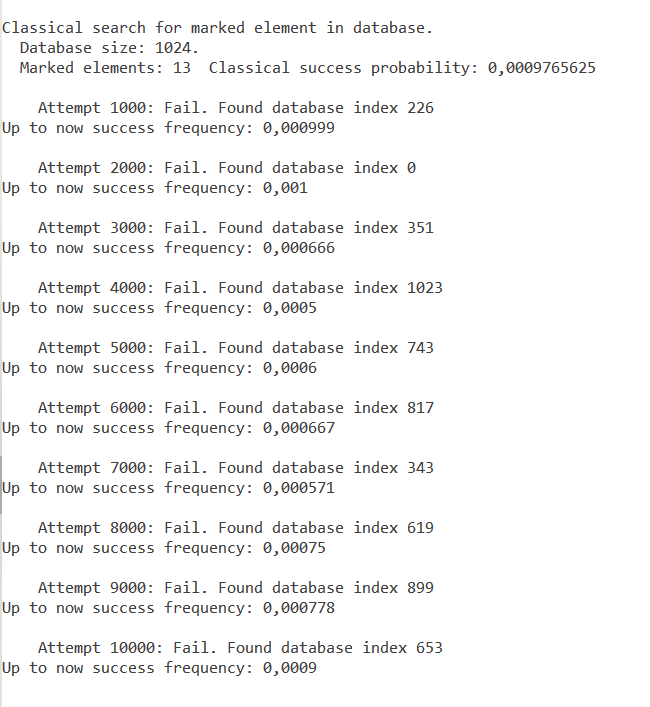
\includegraphics[width=.9\linewidth]{dbsearch_stats1}
	\caption{Classical search on a database. The search complexity is $O(N)$, in fact the probability of picking a the correct element by random choice is $1/N$. In this example the database contains 1024 elements, we look for element 13 and we perform 10 thousands attempts.}
	\label{fig:db_stats1}
\end{figure}

\begin{figure}
	\centering
	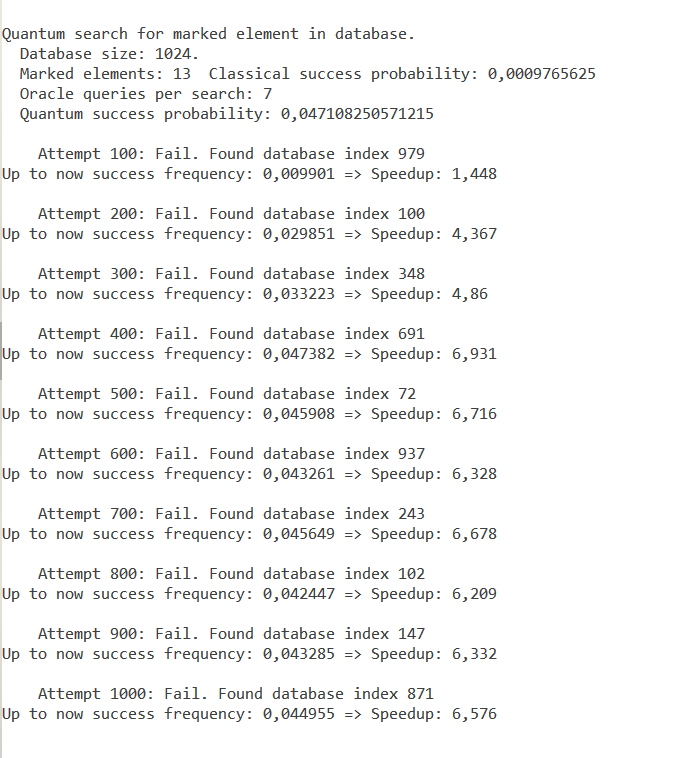
\includegraphics[width=.9\linewidth]{dbsearch_stats2}
		\caption{Quantum search on a database. The search complexity is $O(sqrt{N})$. The quantum success probability is predicted to be higher than the classical one, and the statistics confirm the theory as computed during the attemprs. In this example the database contains 1024 elements, we look for element 13 and we perform 1 thousand attempts (less than classical ones because the simulation of Oracle queries carries some overhead).}
	\label{fig:db_stats2}
\end{figure}

\begin{figure}
	\centering
	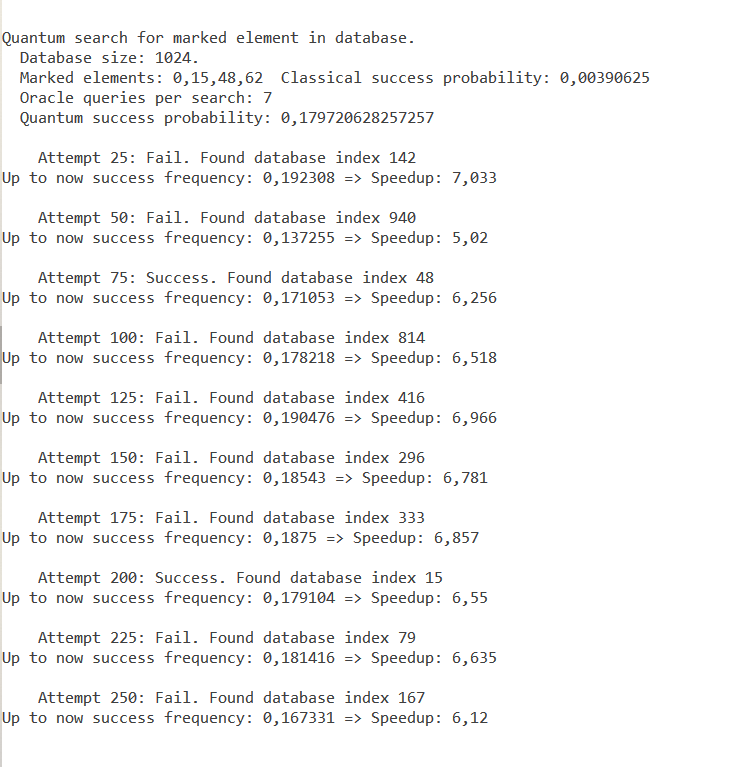
\includegraphics[width=.9\linewidth]{dbsearch_stats3}
	\caption{Again quantum search on a database. The database contains 1024 elements, but this time we look for 4 different elements at the same time. As the simulation gets proportionally heavier, this time we perform 1/4 of the previous attempts, bt enough to confirm the matching between the theoretical success probability and the simulated one.}
	\label{fig:db_stats3}
\end{figure}

\subsection{Possible improvements on this implementation}

In the above code a standard version of Grover's algorithm is discussed. The whole program takes as input only the elements to search, but there is no information about the elements present in the database. In fact the database is implemented through a register of $n$ qubits, that are initialized so that when measured all the values from $0$ to $2^n - 1$ have the same flat probability. In this way the register is actually implementing a virtual database, a mathematical object that has no relevance in real cases as it contains no information. We will focus on this issue in \cref{chp:grover}.